\section{Pengenalan DOM (Document Object Model)}

\textbf{DOM} (Document Object Model) adalah representasi terstruktur dari dokumen HTML sebagai pohon objek yang dapat dimanipulasi oleh JavaScript. Setiap elemen HTML menjadi \textbf{node} di pohon DOM: elemen (\code{<p>}, \code{<div>}), teks, atribut, dan komentar. Browser membangun DOM saat memproses HTML, dan JavaScript dapat membaca serta mengubah DOM secara dinamis---inilah yang membuat halaman web interaktif \cite{mdnJsGuide}.

\begin{figure}[htbp]
\centering
\resizebox{0.8\textwidth}{!}{%
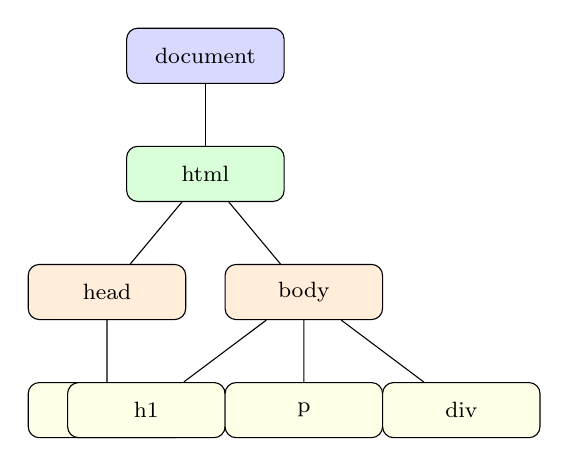
\begin{tikzpicture}[
  every node/.style={font=\footnotesize, draw, rounded corners, minimum width=2cm, minimum height=0.7cm},
  level 1/.style={sibling distance=5cm, level distance=1.5cm},
  level 2/.style={sibling distance=2.5cm, level distance=1.5cm},
  level 3/.style={sibling distance=2cm, level distance=1.5cm}
]
\node[fill=blue!15] {document}
  child { node[fill=green!15] {html}
    child { node[fill=orange!15] {head}
      child { node[fill=yellow!10] {title} }
    }
    child { node[fill=orange!15] {body}
      child { node[fill=yellow!10] {h1} }
      child { node[fill=yellow!10] {p} }
      child { node[fill=yellow!10] {div} }
    }
  };
\end{tikzpicture}%
}
\caption{Pohon DOM: setiap elemen HTML menjadi node}
\end{figure}

Objek global \code{document} adalah titik masuk ke DOM. Dari \code{document}, JavaScript dapat mengakses elemen mana saja menggunakan metode seperti \code{getElementById()}, \code{querySelector()}, dan \code{querySelectorAll()}. Setelah mendapatkan referensi ke elemen, JavaScript dapat mengubah konten, atribut, style, dan bahkan menambah atau menghapus elemen dari halaman \cite{jsInfo}.

\begin{konsep}
\textbf{DOM Bukan HTML.} DOM adalah representasi \textit{live} dari halaman---ia mencerminkan keadaan saat ini, bukan isi file HTML asli. JavaScript yang mengubah DOM tidak mengubah file HTML di server. Browser DevTools (tab Elements) menampilkan DOM saat ini, yang mungkin berbeda dari source HTML jika JavaScript telah memodifikasinya. Memahami perbedaan ini kunci untuk debugging \cite{mdnJsGuide}.
\end{konsep}

